\documentclass[12pt,letterpaper]{article}

\usepackage[hmargin=1in,bottom=1in,top=1in]{geometry}
\usepackage[latin1]{inputenc}
\usepackage{amsmath}
\usepackage{amsfonts}
\usepackage{amssymb}
\usepackage{graphicx}
\usepackage{url}
\usepackage[toc,page]{appendix}
\usepackage{setspace}
\usepackage{pdfpages}

\usepackage{ulem}
\normalem

% push footnotes to the bottom of the page unconditionally
\usepackage[bottom]{footmisc}

\usepackage[pdftex]{hyperref}
\hypersetup{
	pdfauthor={Neil Isaac and Keyi Shi},
	pdftitle={Implementation of a virtual FPGA architecture},
	pdfsubject={Virtual FPGA fabrics},
	colorlinks=true,
	anchorcolor=black,
	linkcolor=blue,
	citecolor=blue,
	filecolor=blue,
	pagecolor=blue,
	urlcolor=blue,
	frenchlinks=false,
	pagebackref=true,
	bookmarks=true}

% make links to figures jump to position above the figure
%\usepackage[all]{hypercap}

%\usepackage{titling}
%\usepackage{listings}
%\lstset{language=c}

% fancyhdr - use top=1.5in
%\usepackage{fancyhdr}
%\pagestyle{fancy}
%\fancyhead[L]{\leftmark}
%\fancyhead[R]{\thepage}
%\fancyhead[CF]{}
%\setlength{\headheight}{16pt}

\setlength{\parindent}{0in}
\setlength{\parskip}{1.0 \baselineskip}
\setlength{\footnotesep}{1.0 \baselineskip}
\setlength{\skip\footins}{2.0 \baselineskip}

\bibliographystyle{IEEEtran}

\usepackage{color}
\newcommand{\note}[1]{}
% comment out the next line to hide draft notes
\renewcommand{\note}[1]{\textcolor{red}{[#1]}}
\newcommand{\citationneeded}[0]{\note{citation needed}}

\newenvironment{enumeration}{
	\setlength{\topsep}{0.0pt}
	\setlength{\partopsep}{0pt}
	\setlength{\parskip}{0pt}
	\setlength{\parsep}{0pt}
	\begin{enumerate}
		\setlength{\itemsep}{0pt}}
	{\end{enumerate}}

\newenvironment{itemlist}{
	\setlength{\topsep}{0pt}
	\setlength{\partopsep}{0pt}
	\setlength{\parskip}{0pt}
	\setlength{\parsep}{0pt}
	\begin{itemize}
		\setlength{\itemsep}{0pt}}
	{\end{itemize}}

\newcommand{\sectref}[1]{Section \ref{#1}}
\newcommand{\figref}[1]{Figure \ref{#1}}
\newcommand{\tableref}[1]{Table \ref{#1}}

%\renewcommand{\thefootnote}{\roman{footnote}}

\begin{document}

\begin{titlepage}
\begin{center}


\includegraphics[scale=1.0]{ecelogo.png}

\vspace{1 \baselineskip}

\textsc{
\Large University of Toronto\\
\large Department of Electrical and Computer Engineering \\
\large ECE496 Design Project
}

\vspace{2 \baselineskip}

{\Large \bfseries Virtual FPGA fabrics} \\
{\Large \bfseries Implementation of a Virtual FPGA Architecture}

\vspace{2 \baselineskip}

{\large \bfseries Final Report} \\

\vspace{2 \baselineskip}

{\large March 22, 2012}

\vfill

\begin{tabular*}{4in}{l @{\extracolsep{\fill}} l}
\textbf{Neil Isaac} & \textbf{Keyi Shi} \\
\texttt{n.isaac@utoronto.ca} & \texttt{keyi.shi@utoronto.ca} \\ & \\
\emph{Project ID:} & 2011017 \\
\emph{Supervisor:} & Jason Anderson \\
\emph{Administrator:} & Ross Gillett \\
\emph{Section:} & \#7 \\
\end{tabular*}

\end{center}
\end{titlepage}



%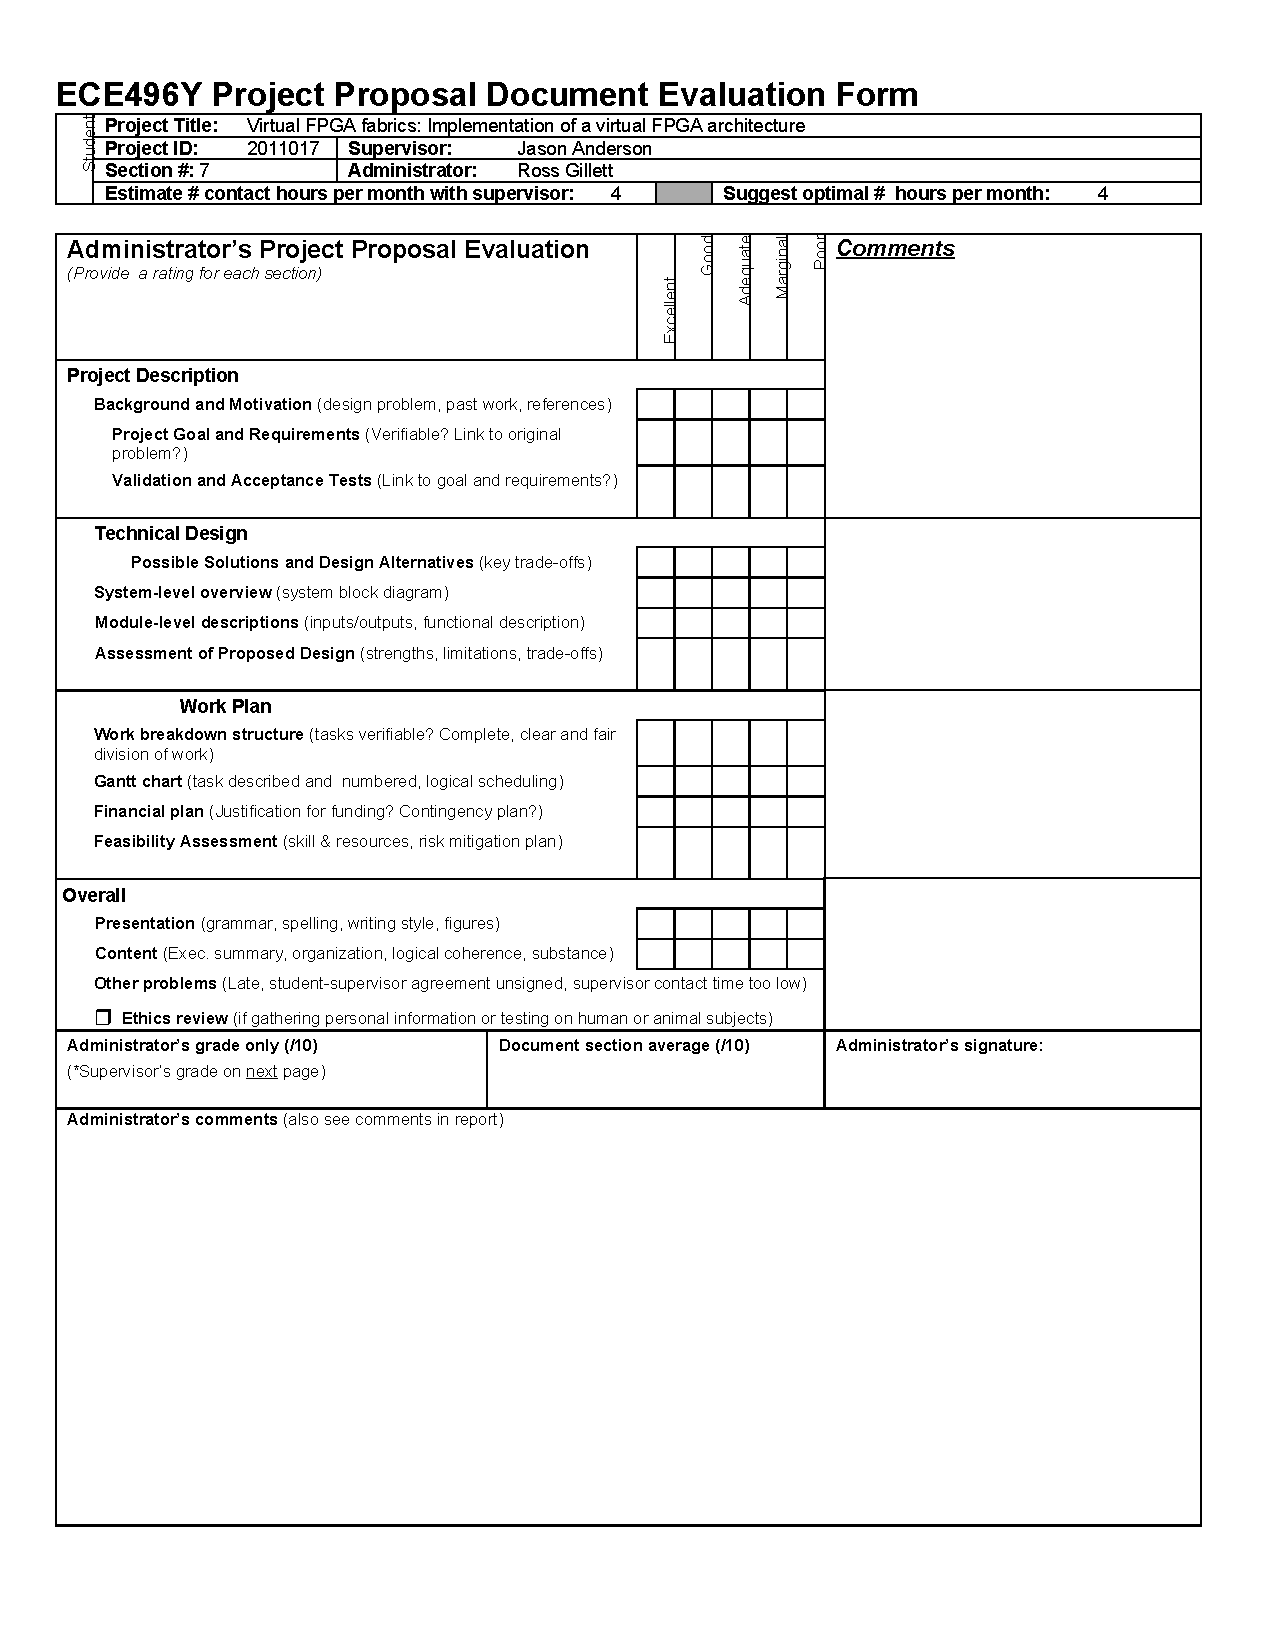
\includepdf{cover1.pdf}
%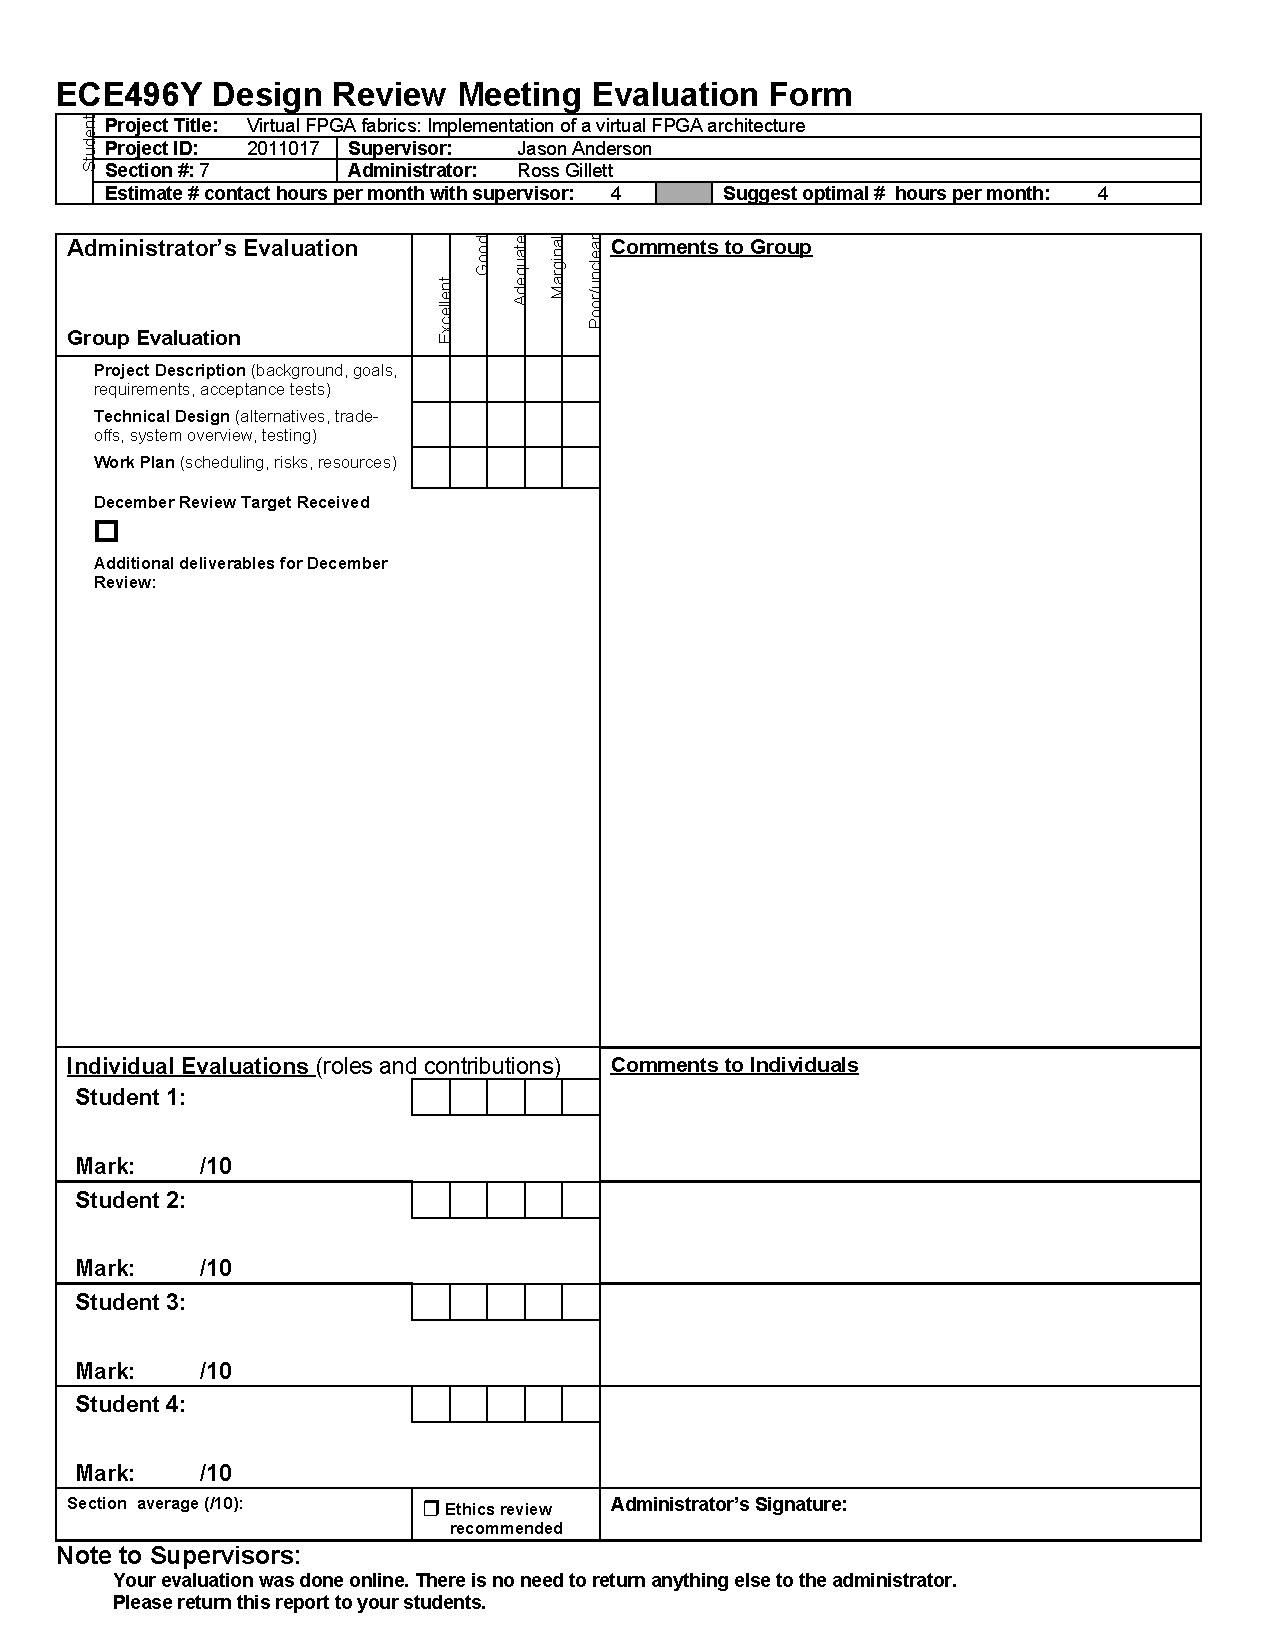
\includepdf{cover2.pdf}

\onehalfspace

%\thispagestyle{empty}
\section*{Executive Summary}

% No more than 1 page
% Should show clear understanding of AUDIENCE and PURPOSE
% Readable as a stand-alone document, clearly differentiated from an introduction
% Give the contest and MOST IMPORTANT information in the document in a unified fashion

Academic studies of Field Programmable Gate Array (FPGA) chip architecture rely on simulations, as commercial FPGA chips contain proprietary designs that make their underlying architecture inaccessible to academic researchers.
The goal of this project is to provide a physical platform for researchers to carry out FPGA architecture studies.
The finished design should capable of running common benchmark circuits.

The proposed design is to implement an Overlay FGPA on an existing, commercially available FPGA chip.
Using a commercial FPGA as the physical medium for this project makes the design cheaper and more accessible to researchers, as they may have an appropriate FPGA chip already.


We have selected the Xilinx Virtex 5 FPGA as our development platform because we can use its native logic units directly.
This will limit the models of FPGA chips that the overlay circuit can be implemented on, but it should reduce the design's area overhead and improve its timing characteristics.
The features we will use on the Virtex 5 are forward-compatible with all current-generation Xilinx FPGA products, allowing the researcher to use a variety of FPGAs.

The validation of the design will involve testing a set of benchmark circuits by placing and routing them with VPR, then transferring them to the FPGA overlay.
The circuits can then be tested for correct behavior, confirming that the overlay design can be correctly programmed using VPR output, and that the inputs and outputs to the design are functioning properly.

The current budget for the proposed design is \$14.00 and will be covered by the students.
The required FPGA development boards and software licenses have been provided by the supervisor.

We have designed and tested the modules required to build one tile of the Overlay FGPA.
By December, we expect to have assembled a grid of tiles and have software support for programming the logic cells.



\pagenumbering{roman}

\singlespace

\setcounter{tocdepth}{1}
\tableofcontents
%\listoffigures
%\listoftables
\pagebreak

\pagenumbering{arabic}

\onehalfspace

\section{Project Overview}

% The intent of this section is to re-introduce the reader to the project. It may be largely crafted
% from previous work if the project has not changed much from the proposal, although it may
% contain details of decisions made since the proposal. As it will set the stage for your progress
% descriptions, you might also want to include information about the main design challenges of
% your project. It must at least create the stage for the individual reports so the relevance of the
% individual work is apparent.
% It is expected that details pertinent to the individual progress will be in the documents from those
% individuals.
% If it makes sense, combine this section with the group progress summary. This section should
% NOT be as detailed as in your Proposal, and may use your Proposal as a reference.


\pagebreak
\section{Group Progress Summary}

% - A summary of the project goal and any changes to the goal or requirements since the
%   design review. A system-level diagram is often helpful. Be brief here since you will also
%   provide an updated copy of the complete project goal and requirements in Appendix B.
%
% - A summary of the group's progress. Highlight a few key accomplishments since the
%   design review. Briefly describe some of the key challenges that were encountered and
%   some of the key decisions that were made in this time. Is the group on schedule? Make
%   explicit reference to the milestones on the original Gantt chart from the Project Proposal.
%
% - The key responsibilities of each team member since the design review. One or two items
%   for each member is sufficient, and can be general areas instead of tasks.
%
% - A summary of any changes to the group work plan, individual responsibilities, or the
%   project milestones. Again, be brief here since you will provide the details in Appendix A.


%% timeline - nothing else related to project management has changed (goals, work plan, etc) - maybe we should say that explicitly. %%
Our project is progressing well and we are optimistic that we can meet our deadlines.
We initially planned optimistic deadline for long-term tasks, but left a couple of months of slack at the end of the project.
Now that we have begun those tasks, we have adjusted the gantt chart to reflect more realistic expectations for some of those tasks.
The slack time is now reflected within the time allocations for the tasks themselves.
The updated gantt chart is included in Appendix \ref{new-gantt-chart}, and the old version is in Appendix \ref{old-gantt-chart}.

%% tasks - could add our names to them to reflect bullet 3 above? %%
In order to build a working \emph{Overlay FPGA}, we need to produce the following:
\begin{itemize}
\item Verilog for the individual FPGA building-blocks: the logic cell, logic block, connection block, and the switch block.
\item Verilog to connect the building block components together in a grid and feed the programming signals through them.
\item Verilog circuit to interface with the UART to enable serial programming of the Overlay FPGA.
\item Scripts to run the third-party tools which will process an input circuit (from the user) and produce a valid placment and routing. Some adjustments need to be made so the tools can read each others' outputs.
\item Software to convert the placement and routing into a programmable bitstream.
\end{itemize}


%% rest is status on tasks %%

We have completed the building-block components of the design, and the components all work individually, but need to do extensive debugging work to get it all working together.

The software is also complete, but can't be fully tested until the hardware is fully functional.
Partial validation was done on the software by manually reading the bitstream file it produces.

Once we complete this debugging, we have a number of improvements planned to improve the quality of the virtual FPGA (in terms of usability to researchers, as well as its efficiency.)
These improvements are not necessary for a proof-of-concept, or for a fully functional demo.

We are confident that we can complete these remaining tasks before the design fair.





%\pagebreak
%%\nocite{*} % show uncited entries in the bibliography
%\bibliography{ref}
%\addcontentsline{toc}{section}{References}

\pagebreak
\begin{appendices}
\section{Gantt Chart}
\label{gantt-chart}

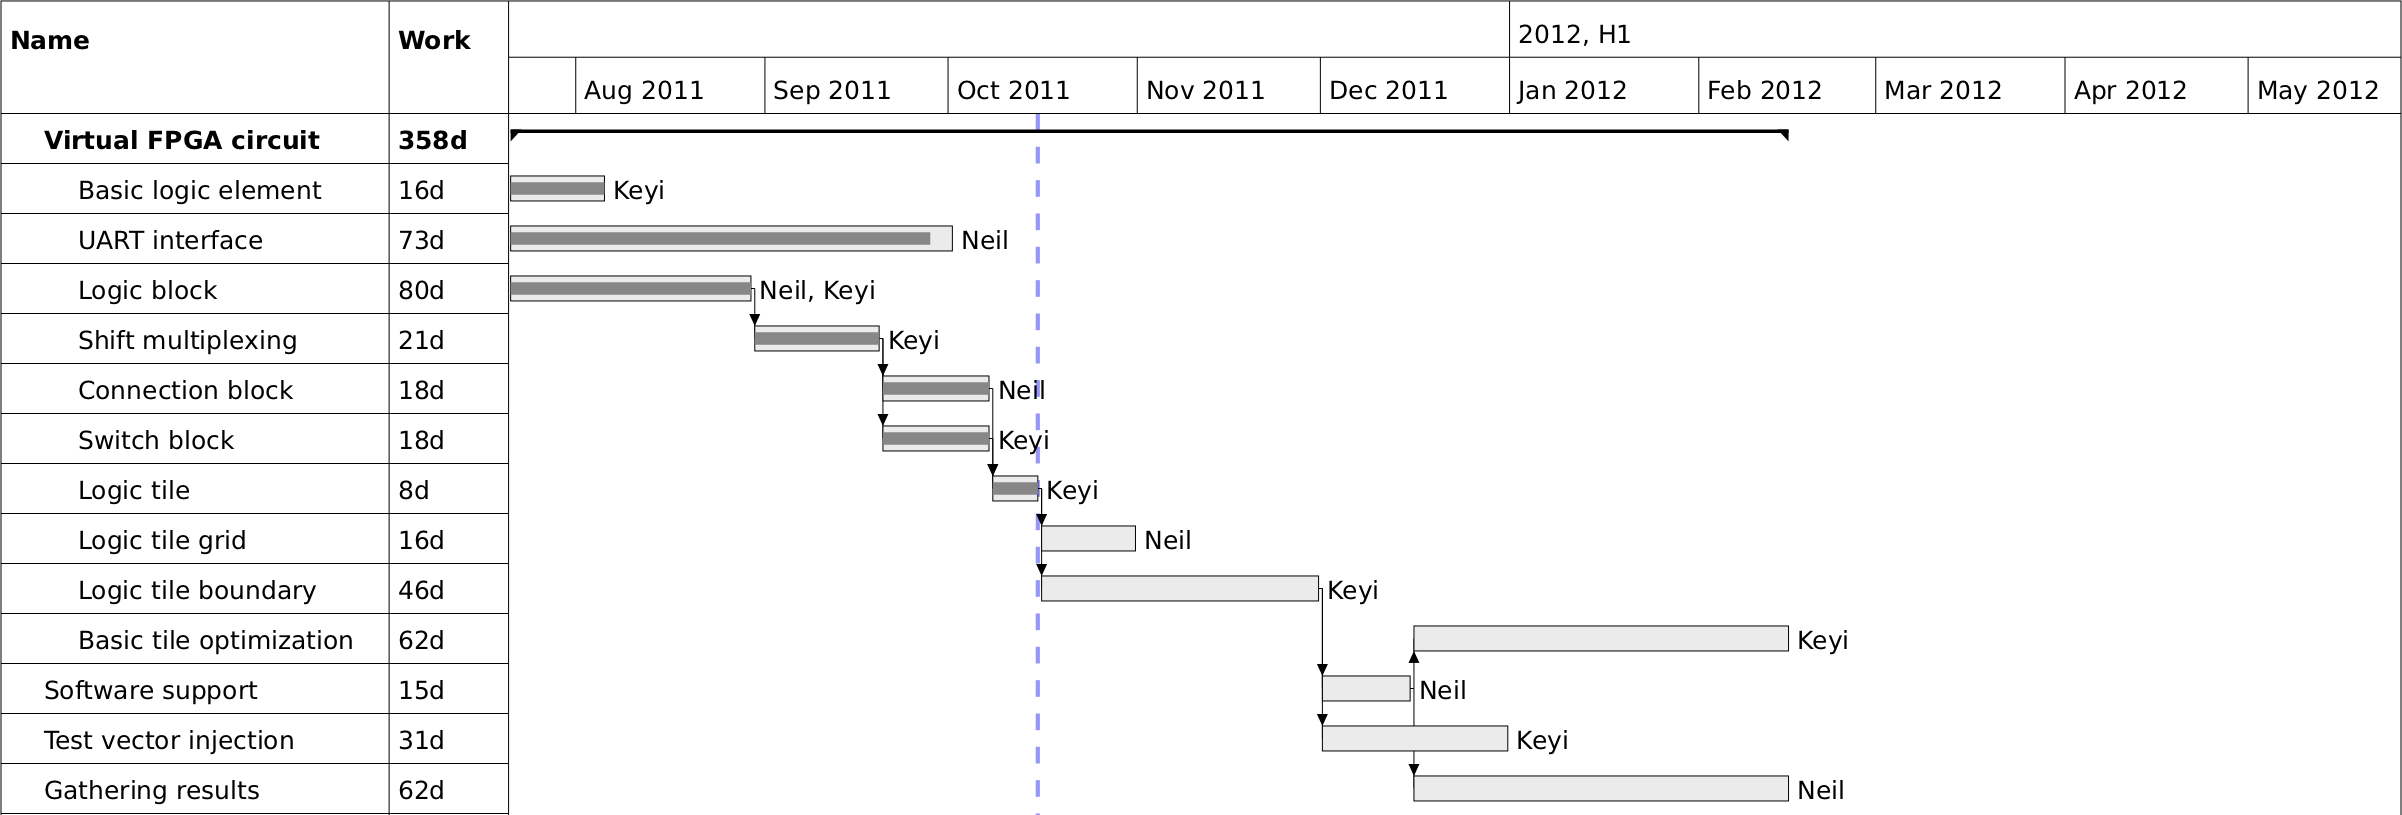
\includegraphics[scale=0.45,angle=90]{gantt.png}


\section{Project Goals and Requirements}

% Insert a copy of the „Project Goal‟ and „Project Requirements‟ sections from the Project
% Proposal. If there are any changes, briefly justify the changes and provide an updated version of
% the current Project Goals and Requirements.

% I just copied this from the final proposal.  We may want to simplify it for the presentation.


\subsection{Functional Requirements}

An Overlay FGPA circuit that will:

\begin{itemlist}
	\item Work on a commercially available FPGA chip.
	\item Be re-programmable over a serial interface after being flashed to the FPGA.
	\item Have a tunable number and arrangement of logic cells, and have tunable connectivity parameters. 
	\item Support inputs to and outputs from test circuits programmed onto the Overlay FGPA.
\end{itemlist}

A software program that can:
\begin{itemlist}
	\item Translate VPR placement and routing data for a test circuit into a bitstream for the Overlay FGPA.
	\item Program the bitstream onto the Overlay FGPA to implement the circuit.
\end{itemlist}

\subsection{Constraints}

\begin{itemlist}
	\item The overlay circuit must support at least 3000 logic cells\footnote{3000 logic cells was chosen as the minimum target because the largest of the ``Golden 20'' circuits, \emph{``s38417''} requires 2567 6-input logic cells\cite{synthesis-density}.} in order to accommodate the \emph{``Golden 20''} MCNC benchmark circuits\footnote{The ``Golden 20'' MCNC circuits are available in BLIF format at \url{http://www.ece.ubc.ca/~julienl/benchmarks.htm}.} commonly used in FPGA research.
\end{itemlist}


\subsection{Objectives}

\begin{itemlist}
	\item Be compatible with a family of commercial FPGAs that are available to researchers.
	\item Use the native logic cells in the physical FPGA directly in the overlay FPGA design to reduce area and latency.
	\item Be fast enough that it outperforms software emulation of most test circuits.
\end{itemlist}


\end{appendices}

%\pagebreak
%\fancyhead[L]{Addenda}
%\addcontentsline{toc}{section}{Title}
%\section*{Title}
%\input{file}
%\pagebreak

\end{document}

